\documentclass[]{jarticle}          % 一段組
%\documentclass[twocolumn]{jarticle} % 二段組

\textwidth 180mm
\textheight 255mm
\oddsidemargin -12mm
\topmargin -15mm
\columnsep 10mm

%\vspace{0.5cm} % 一段組の場合はコメントアウトした方が体裁がよいx
%] % 一段組の場合はコメントアウトする

\usepackage{styles/labheadings}
\usepackage[dvipdfmx]{graphicx,color}
\usepackage{amsmath,amssymb}
\usepackage{url}
% 追加
\usepackage[hang,small,bf]{caption}
\usepackage[subrefformat=parens]{subcaption}
\captionsetup{compatibility=false}

\newcommand{\aU}{\mbox{\boldmath $a$}}
\newcommand{\bU}{\mbox{\boldmath $b$}}
\newcommand{\cU}{\mbox{\boldmath $c$}}
\newcommand{\dU}{\mbox{\boldmath $d$}}
\newcommand{\eU}{\mbox{\boldmath $e$}}
\newcommand{\fU}{\mbox{\boldmath $f$}}
\newcommand{\gU}{\mbox{\boldmath $g$}}
\newcommand{\hU}{\mbox{\boldmath $h$}}
\newcommand{\iU}{\mbox{\boldmath $i$}}
\newcommand{\jU}{\mbox{\boldmath $j$}}
\newcommand{\kU}{\mbox{\boldmath $k$}}
\newcommand{\lU}{\mbox{\boldmath $l$}}
\newcommand{\mU}{\mbox{\boldmath $m$}}
\newcommand{\nU}{\mbox{\boldmath $n$}}
\newcommand{\oU}{\mbox{\boldmath $o$}}
\newcommand{\pU}{\mbox{\boldmath $p$}}
\newcommand{\qU}{\mbox{\boldmath $q$}}
\newcommand{\rU}{\mbox{\boldmath $r$}}
\newcommand{\sU}{\mbox{\boldmath $s$}}
\newcommand{\tU}{\mbox{\boldmath $t$}}
\newcommand{\uU}{\mbox{\boldmath $u$}}
\newcommand{\vU}{\mbox{\boldmath $v$}}
\newcommand{\wU}{\mbox{\boldmath $w$}}
\newcommand{\xU}{\mbox{\boldmath $x$}}
\newcommand{\yU}{\mbox{\boldmath $y$}}
\newcommand{\zU}{\mbox{\boldmath $z$}}
\newcommand{\AU}{\mbox{\boldmath $A$}}
\newcommand{\BU}{\mbox{\boldmath $B$}}
\newcommand{\CU}{\mbox{\boldmath $C$}}
\newcommand{\DU}{\mbox{\boldmath $D$}}
\newcommand{\EU}{\mbox{\boldmath $E$}}
\newcommand{\FU}{\mbox{\boldmath $F$}}
\newcommand{\GU}{\mbox{\boldmath $G$}}
\newcommand{\HU}{\mbox{\boldmath $H$}}
\newcommand{\IU}{\mbox{\boldmath $I$}}
\newcommand{\JU}{\mbox{\boldmath $J$}}
\newcommand{\KU}{\mbox{\boldmath $K$}}
\newcommand{\LU}{\mbox{\boldmath $L$}}
\newcommand{\MU}{\mbox{\boldmath $M$}}
\newcommand{\NU}{\mbox{\boldmath $N$}}
\newcommand{\OU}{\mbox{\boldmath $O$}}
\newcommand{\PU}{\mbox{\boldmath $P$}}
\newcommand{\QU}{\mbox{\boldmath $Q$}}
\newcommand{\RU}{\mbox{\boldmath $R$}}
\newcommand{\SU}{\mbox{\boldmath $S$}}
\newcommand{\TU}{\mbox{\boldmath $T$}}
\newcommand{\UU}{\mbox{\boldmath $U$}}
\newcommand{\VU}{\mbox{\boldmath $V$}}
\newcommand{\WU}{\mbox{\boldmath $W$}}
\newcommand{\XU}{\mbox{\boldmath $X$}}
\newcommand{\YU}{\mbox{\boldmath $Y$}}
\newcommand{\ZU}{\mbox{\boldmath $Z$}}
\newcommand{\epU}{\mbox{\boldmath $\epsilon$}}
\newcommand{\taU}{\mbox{\boldmath $\tau$}}
\newcommand{\etU}{\mbox{\boldmath $\eta$}}
\newcommand{\xiU}{\mbox{\boldmath $\xi$}}
\newcommand{\wwU}{\mbox{\boldmath $\omega$}}
\newcommand{\WwU}{\mbox{\boldmath $\Omega$}}
\newcommand{\lmU}{\mbox{\boldmath $\lambda$}}
\newcommand{\LmU}{\mbox{\boldmath $\Lambda$}}
\newcommand{\PiU}{\mbox{\boldmath $\Pi$}}
\newcommand{\SgU}{\mbox{\boldmath $\Sigma$}}
\newcommand{\thU}{\mbox{\boldmath $\theta$}}
\newcommand{\ThU}{\mbox{\boldmath $\Theta$}}
\newcommand{\roU}{\mbox{\boldmath $\rho$}}
\newcommand{\nuU}{\mbox{\boldmath $\nu$}}
\newcommand{\ones}{{\bf 1}}
\newcommand{\zr}{{\bf 0}}
\newcommand{\eq}{\begin{equation}}
\newcommand{\en}{\end{equation}}
\newcommand{\eqa}{\begin{eqnarray}}
\newcommand{\ena}{\end{eqnarray}}
\newcommand{\xx}{\makebox[1cm]{}}
\newcommand{\xm}{\makebox[0.5cm]{}}
\newcommand{\x}{\makebox[0.2cm]{}}
\newcommand{\tr}{{\rm tr}}
\newcommand{\sgn}{{\rm sgn}}
\newcommand{\ad}{{\rm ad}}
\newcommand{\rank}{{\rm rank}}
\newcommand{\diag}{{\rm diag}}
\newcommand{\lbr}{\left(\begin{array}}
\newcommand{\rbr}{\end{array}\right)}
\newcommand{\Proof}{\noindent{\em Proof\/}}
\newcommand{\Solution}{\noindent{\em Solution}}
\newcommand{\Derivation}{\noindent{\em Derivation}}
\newcommand{\msp}{\vspace*{\medskipamount}\\}
\newcommand{\qed}{\hspace*{\fill}$\Box$}
\newcommand{\aX}{{\bf a}}
\newcommand{\bX}{{\bf b}}
\newcommand{\cX}{{\bf c}}
\newcommand{\dX}{{\bf d}}
\newcommand{\eX}{{\bf e}}
\newcommand{\fX}{{\bf f}}
\newcommand{\gX}{{\bf g}}
\newcommand{\hX}{{\bf h}}
\newcommand{\iX}{{\bf i}}
\newcommand{\jX}{{\bf j}}
\newcommand{\kX}{{\bf k}}
\newcommand{\lX}{{\bf l}}
\newcommand{\mX}{{\bf m}}
\newcommand{\nX}{{\bf n}}
\newcommand{\oX}{{\bf o}}
\newcommand{\pX}{{\bf p}}
\newcommand{\qX}{{\bf q}}
\newcommand{\rX}{{\bf r}}
\newcommand{\sX}{{\bf s}}
\newcommand{\tX}{{\bf t}}
\newcommand{\uX}{{\bf u}}
\newcommand{\vX}{{\bf v}}
\newcommand{\wX}{{\bf w}}
\newcommand{\xX}{{\bf x}}
\newcommand{\yX}{{\bf y}}
\newcommand{\zX}{{\bf z}}
\newcommand{\AX}{{\bf A}}
\newcommand{\BX}{{\bf B}}
\newcommand{\CX}{{\bf C}}
\newcommand{\DX}{{\bf D}}
\newcommand{\EX}{{\bf E}}
\newcommand{\FX}{{\bf F}}
\newcommand{\GX}{{\bf G}}
\newcommand{\HX}{{\bf H}}
\newcommand{\IX}{{\bf I}}
\newcommand{\JX}{{\bf J}}
\newcommand{\KX}{{\bf K}}
\newcommand{\LX}{{\bf L}}
\newcommand{\MX}{{\bf M}}
\newcommand{\NX}{{\bf N}}
\newcommand{\OX}{{\bf O}}
\newcommand{\PX}{{\bf P}}
\newcommand{\QX}{{\bf Q}}
\newcommand{\RX}{{\bf R}}
\newcommand{\SX}{{\bf S}}
\newcommand{\TX}{{\bf T}}
\newcommand{\UX}{{\bf U}}
\newcommand{\VX}{{\bf V}}
\newcommand{\WX}{{\bf W}}
\newcommand{\XX}{{\bf X}}
\newcommand{\YX}{{\bf Y}}
\newcommand{\ZX}{{\bf Z}}

% report.texと同じディレクトリにnumerical_definition.texを入れておけば上の書き方でもいいはずです

\usepackage[
  dvipdfm,
  bookmarks=true,
  bookmarksnumbered=true,
  colorlinks=true]{hyperref}
\AtBeginDvi{\special{pdf:tounicode EUC-UCS2}}

\pagestyle{labheadings}
\headerleft{2次元フロアマップからのシーンの3次元モデルの作成}   % ヘッダの左側のタイトル
\headerright{2024年9月4日}  % ヘッダの右側のタイトル

\begin{document}

%\twocolumn % 一段組の場合はコメントアウトする

\vspace*{2ex}
\begin{center}
 {\Large \bf 複数の全方位画像を持ちいた三次元モデルのテクスチャ貼り付け}\\ % タイトル
 \vspace*{5mm}
 {\large M1 田川幸汰}% 発表者名
\end{center}

%\vspace{0.5cm} % 一段組の場合はコメントアウトした方が体裁がよいx
%] % 一段組の場合はコメントアウトする

%新しく作成したコマンド
% \newcommand{\reffig}[1]{\hyperref[#1]{図\ref{#1}}}
% \newcommand{\refeq}[1]{\hyperref[#1]{式(\ref{#1})}}
% \newcommand{\reftab}[1]{\hyperref[#1]{表\ref{#1}}}
% \newcommand{\refsec}[1]{\hyperref[#1]{\ref{#1}章}}
% \newcommand{\refsubsec}[1]{\hyperref[#1]{\ref{#1}節}}

% 数式
%\begin{equation}
%  数式記述  
%  \label{ラベル名}
%\end{equation}

% 図
% \begin{figure}[!ht]
%   \begin{center}
%     \includegraphics[scale=0.5]{figures/画像ファイル名}
%     \caption{キャプション名}
%     \label{ラベル名}
%   \end{center}
% \end{figure}

% リスト
% \begin{enumerate or itemize}
%   \item 
% \end{enumerate or itemize}
\section{概要}
前回の進捗報告では単一の全方位画像を使用して3次元モデルのテクスチャ貼り付けを行った。
しかし、単一の全方位画像では三次元モデルの面までの距離や、角度等の理由でテクスチャを取得できない面がある。
そのため、複数の全方位画像からテクスチャを取得してより多くの面のテクスチャを取得できるようにする。

\section{複数の全方位画像からテクスチャを取得し、3次元モデルに貼り付け}
\subsection{実装方法}
3次元モデルに対して、正しい大きさ、位置、方向でテクスチャを割り当てる。
3次元モデルの三角形メッシュの重心に対してカメラの視線を向けるように、
全方位画像から作成した透視投影画像を用いてテクスチャを取得する。
以下に、テクスチャを取得する具体的な手順を示す。
\begin{enumerate}
  \item メッシュを構成する3点をカメラの外部パラメータを用いて世界座標系からカメラ座標系に変換する。
  \item メッシュの重心ベクトルを計算する。
  \item メッシュの重心ベクトルの大きさがしきい値以内のメッシュに対して以下の処理を行う。
  \item 重心ベクトルの仰角$\phi$の値を計算する。
  \item 仰角の大きさがしきい値以内のメッシュに対して以下の処理を行う。
  \item カメラの視線ベクトルがメッシュの重心を向くような回転行列を計算し、三角形メッシュの座標を変換する。
  \item カメラの内部パラメータを用いて三角形メッシュの座標を透視投影画像に投影する。
  \item メッシュを構成する3点が画像面上に収まっている場合、全方位画像から透視投影画像を作成する。
  \item テクスチャが未割り当ての場合はテクスチャを割り当て、3次元モデルを更新する。
  \item テクスチャが割り当てられている場合は、重心ベクトルの大きさを比較してより小さい方をテクスチャとして採用する。
\end{enumerate}
前回の進捗報告からの主な変更点は、4、5、9、10の項目である。
4と5の処理を追加した理由は、全方位カメラの下部にスタンドなどが映り込み、テクスチャに不適切な要素が含まれるのを防ぐためである。
具体的には、カメラが映り込むような角度のテクスチャを除外することで、より正確なテクスチャ割り当てを実現する。
また、9と10の処理を追加した理由は、複数の全方位画像を使用して、より精度の高いテクスチャを取得するためである。
これにより、既に割り当てられたテクスチャが不十分なメッシュに対して、
追加の全方位画像からのより良いテクスチャを割り当てることが可能になる。

また、前回の進捗報告では一つのメッシュのサイズが大きすぎて、透視投影画像に写りきらないという問題があったため、
3次元モデルを頂点数を増やし、より細かいメッシュになるよう作り直した。

\subsection{実装結果}
テクスチャを取得し、3次元モデルに貼り付けた結果を\hyperref[one]{図\ref{one}}に示す。
\begin{figure}[!ht]
  \begin{center}
    \begin{tabular}{cc}
      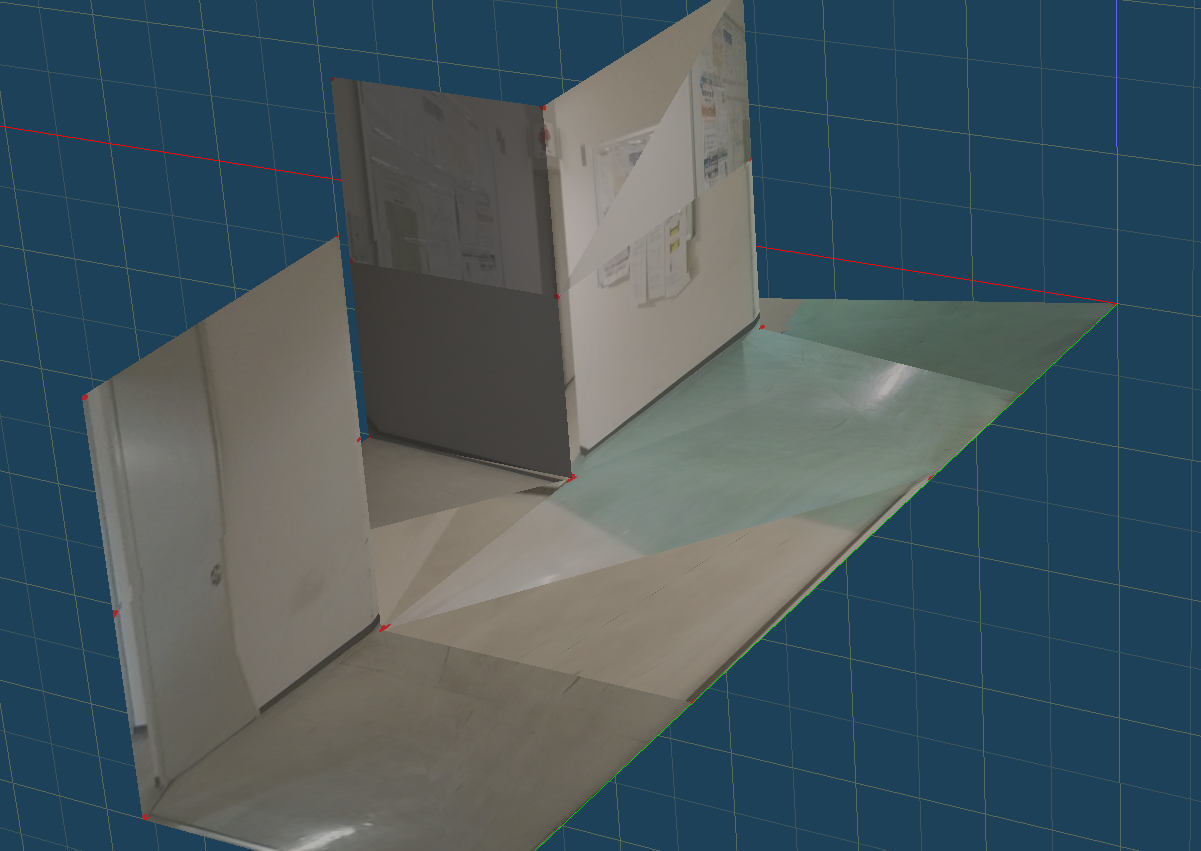
\includegraphics[keepaspectratio, scale=0.3]{figures/3dmodel1.png}\\
      (a)3次元モデル前面\\
      \\
      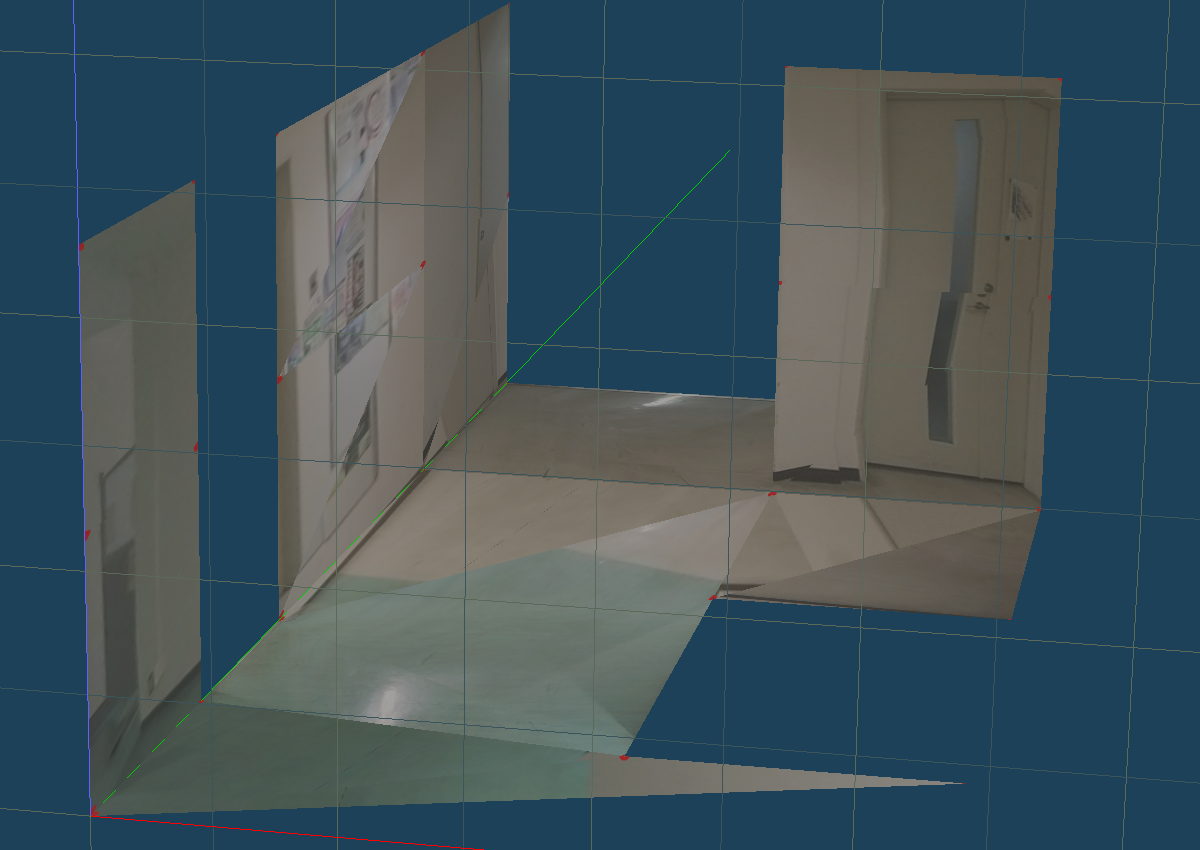
\includegraphics[keepaspectratio, scale=0.3]{figures/3dmodel2.png}\\
      (b)3次元モデル後面\\
    \end{tabular}
  \end{center}
  \caption{出力結果}
  \label{one}
\end{figure}
前回の進捗報告からの進捗として、複数の全方位画像を用いたこと、メッシュのサイズをより細かくしたことで
すべてのメッシュにテクスチャを割り当てることができている。
また、前回の進捗報告で見られた障害物越しのテクスチャを取得してしまうという問題は、
複数の全方位画像を用いることである程度は解決されている。

しかし、異なる全方位画像を用いたテクスチャのつなぎ目が不完全になっていることがわかる。
これは、カメラごとに外部パラメータが正しく取得できていないことが理由だと考えられる。しかし、推定精度には限界があるため、
外部パラメータの精度向上と並行して、つなぎ目を滑らかにする方法を考察する必要がある。

\section{全方位カメラ位置姿勢の推定結果を用いたテクスチャ貼り付け}

現在、全方位カメラの位置姿勢推定とその結果を基にしたテクスチャの貼り付けを進めている。

全方位カメラ位置姿勢について、シミュレーションデータを用いた場合には正確な位置姿勢を推定できることが
既に確認されているが、実際のデータに適用した際には、正確なカメラ位置姿勢を推定することができていない状況である。

\begin{figure}[!ht]
  \begin{center}
    \begin{tabular}{c}
      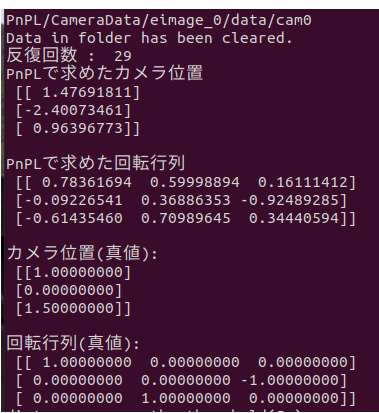
\includegraphics[keepaspectratio, scale=0.5]{figures/kekka.png}
    \end{tabular}
  \end{center}
  \caption{全方位カメラの推定結果}
  \label{two}
\end{figure}

まず、シミュレーションデータでの成功例に対して、実データでの失敗の要因を考える。
シミュレーションデータでは、3次元座標とそれを射影変換した2次元座標を推定に利用していて、仮想カメラ(透視投影画像)の数も最適に設定されている。
しかし、実データを使用する際には、2次元座標は全方位画像から生成した透視投影画像から取得するように変更していて、
この変更がプログラムの実装に何らかの問題を引き起こしている可能性が考えられる。

さらに、実データにおいて2次元座標取得に使用している透視投影画像の数が、
シミュレーションデータで使用した仮想カメラの数よりも少ないことが、問題を引き起こしている可能性も考えられる。
仮想カメラの数が少ないと、全方位カメラの位置姿勢推定に必要な視点情報が不足し、
推定結果に影響を与える可能性がある。

\subsection{今後の目標}
まずプログラムの実装に問題がないかを徹底的に検証することが必要である。
また、使用する透視投影画像の数や視線方向を再評価し、最適な設定を模索することも重要である。
今月中にこれらの問題点を解決し、全方位カメラの正確な位置姿勢推定を行ったうえで、
テクスチャの貼り付けを実現することを目指す。

また、現在はモデルの3次元座標に対応する透視投影画像上の2次元座標を手動で取得しているが、
これを自動化したいと考えている。具体的には、画像上の特徴点を自動で検出し、
それを3次元座標と対応付けるシステムを構築する。この自動化によって、作業の効率化が期待されるが、
カメラの位置姿勢の精度がどうなるかについては検証する必要がある。
\end{document}
